
\documentclass[a4paper,11pt, twocolumn]{article}
\usepackage[utf8]{inputenc}
\usepackage[T1]{fontenc}
\usepackage[norsk]{babel}
\usepackage{graphicx} %for å inkludere grafikk
\usepackage{verbatim} %for å inkludere filer med tegn LaTeX ikke liker
\usepackage{mathpazo}
\usepackage{mathtools}
\usepackage{csquotes}
\usepackage{tikz}
\usepackage{circuitikz}
\usepackage{listings}
\usepackage{booktabs}
\usepackage{todonotes}
\usepackage[backend=biber]{biblatex}
\usepackage[font =small,it]{caption} 
\usepackage{parboxx}
\usepackage{multirow}
\usetikzlibrary{decorations.markings}
\hyphenpenalty=750
\captionsetup[table]{skip=10pt}
\addbibresource{magnetisering.bib}

\lstset{language=Matlab, commentstyle=\textcolor[rgb]{0.00,0.50,0.00}, keepspaces=true, columns=flexible, basicstyle=\footnotesize, keywordstyle=\color{blue}, showstringspaces=false, inputencoding=ansinew}

\title{Magnetisme\\ FYS2150}

\author{Eivind Brox}
\date{\today}

\begin{document}
\tikzset{->-/.style={decoration={markings, mark=at position #1 with {\arrow[scale=3]{stealth reversed}}},  postaction={decorate}}}\maketitle

\tikzset{-<-/.style={decoration={markings, mark=at position #1 with {\arrow[scale=3]{>}}},  postaction={decorate}}}\maketitle



\begin{abstract}
\end{abstract}

\section{Introduksjon}
Det er fire partielle ligninger som ligger til grunn for den klassiske elektromagnetiske teorien. Matematisk er Maxwells ligninger, som de blir kalt, fullt symmetriske i forhold til magnetiske og elektriske fenomener. I virkeligheten finner vi likevel små forskjeller som kommer av at det finnes elektriske, men ikke magnetiske monopoler.

Magnetfelt dannes av elektriske ladninger i bevegelse. Disse mikroskopiske bevegelsene danner grunnlaget for lukkede magnetfeltlinjer som vi kan observere effekten av fra det makroskopiske perspektiv. 

En nyttig del av elektromagnetismen er å karakterisere de magnetiske egenskapene til forsjellige materialer. Elektronets spinn spiller en sentral rolle i forklaringen av de magnetiske egenskapene til mange materialer. Vi skiller mellom banespinn og egenspinn. Banespinn er en egenskap elektroner har når de er bundet til atomkjerne, og den fører til et bidrag til atomets totale magnetiske moment. Egenspinn, en velkjent egenskap i kvantemekanikken, fører til at elektronet i seg selv fungerer som en svakt magnetisk dipol.

Vi skiller mellom tre hovedformer for magnetiske materialer. Disse har egenskaper som avhenger av om banespinnene innad i atomene kansellerer hverandre eller ikke. I denne teksten introduseres først disse forskellige formene for magnetisk materiale. Etter dette følger endel teori som blir nyttig i forhold til eksperimentene som er skissert i seksjonen etter.

\todo[inline]{Gjøre ferdig oversikt}

\section{Teori}
Det meste av teorien er et forsøk på å forkorte og ta med det essensielle fra oppgaveteksten~\cite{oppgavesett}, i forhold til eksperimentene som ble utført.
\subsection{Maxwells ligninger}
En tidlig form av Maxwells ligninger ble publisert mellom 1861 og 1862, og idag skrives de gjerne på differential form~\cite[kap. 9.3.3]{griffithsED}
i
\begin{align}
	&\nabla\cdot\mathbf{E}= \frac{\rho}{\epsilon_0}
	\label{eq:max1}\\
	&\nabla\cdot\mathbf{B} = 0
	\label{eq:max2}\\
	&\nabla\times\mathbf{E} = -\frac{\partial \mathbf{B}}{\partial t}
	\label{eq:max3}\\
	&\nabla\times\mathbf{B} = \mu_0\mathbf{J}+\mu_0\epsilon_0\frac{\partial\mathbf{E}}{\partial t}
	\label{eq:max4}
\end{align}

Her er $\mathbf{E}$ og $\mathbf{B}$ henholdsvis det elektriske og det magnetiske vektorfeltet, $\mu_0$ er den magnetiske permieabiliteten og $\epsilon_0$ er den elektiske permititiviteten $\rho$ er ladningstetthet i vakuum. Strømtetthetten $\mathbf{J}$ er definert slik at 
\begin{equation}
	I = \int_\Omega \mathbf{J}\cdot d\mathbf{a}
	\label{eq:currentDensity}
\end{equation}

der $I$ er den totale strømmen gjennom en lukket flate $\Omega$ med den infinitesimale flateelementvektoren $d\mathbf{a}$ normalt på flatens tangentplan, pekende i motsatt retning av krumningsradiens sentrum. 
\subsection{Diamagnetisme}
De \textit{diamagnetiske} materialene består av atomer der elektronenes spinn kanselleres. Dette er det mest vanlige ettersom elektroner i par helst har motsatt rettet spinn. Dette materialet er altså ikke magnetisk i seg selv. Påfører vi materialet et magnetisk felt vil det det derimot sette opp et lite magnetisk felt som er rettet slik at det setter opp en \textit{Lorentzkraft} som er rettet slik at frorandringene i det magnetiske feltetet i materiale motsettes. Vi sier at diamagnetiske materialer har negativ suceptibilitet, $\chi <0$, og grunnet kraften som settes opp når de føres inn i et magnetfelt, så blir de presset ut av feltet.

Denne egenskapen gjelder for alle atomer, men siden den diamagnetiske effekten er svært liten vil den i enkelte tilfeller utkonkurreres av andre effekter. Slike effekter ser vi nærmer på i neste seksjon.

\subsection{Para- og ferromagnetisme}
Motsetningen til diamagnetiske materialer finner vi i materialer der elektroner opptrer uparrede. I disse tilfellene får atomene et netto spinn og dermed et netto magnetisk moment, ${\boldsymbol \mu}$, slik at hvert atom fungerer som en liten stavmagnet. Dersom atomene i stoffet ikke er orientert tilfeldig vil vi kunne observere magnetfelt utenfor materialet.

Magnetiseringen til et materiale definerer vi som
\begin{equation}
	\mathbf{M} = \frac{d {\boldsymbol \mu}}{dV}
	\label{eq:magnetization}
\end{equation}

hvor totalt magnetisk moment for materialet er integralet til magnetiseringen over volumet til materialet,

\begin{equation}
	{\boldsymbol \mu} = \iiint \mathbf{M}dV
	\label{eq:totalMoment}
\end{equation}

Innefor kategorien av materialer med uparrede elektroner finner vi blant annet de som bare er magnetisert når de påtrykkes ytre magnetfelt. De magnetiserte atomene vil minimere sin energi, og retter seg derfor etter det påtrykte magnetfeltet. Magnetiseringen er proporsjonal med det påtrykte feltet, og vi skriver 
\begin{equation}
	\mathbf{M} = \chi\mathbf{H}
	\label{eq:proposjonalitetPara}
\end{equation}
der $\mathbf{H}$ er det påtrykte magnetfeltet. Den magnetiske suceptibiliteten, $\chi$, for paramagnetiske materialer, som disse materialene kalles, ligger i området $0<\chi<<1$. Den ekstra magnetiseringen som framkommer ved å tilføre et paramagnetisk materiale i et ytre magnetfelt gjør det naturlig å betrakte disse materialene som små magnetfeltforsterkere.

Noen materialer med uparrede elektroner oppfører seg på omtrent samme måte som paramagnetiske materialer, men har en mye større evne til å forsterke det påtrykte magnetfeltet. Disse materialene kalles \textit{ferromagnetiske}, og de inbyrdes atomene har så sterke vekselvirkninger, at etter å ha vært utsatt for et midlertidig magnetfelt, så kan orienterigen til atomene fortsatt være slik at materialets magnetisering også viser seg utenfor materialet. 

\subsubsection{B- og H-felt}
I mange tilfeller er det nyttig å benytte forskjellige former for magnetiske felt. $B$-feltet er summen av alle de magnetiske effektene og kalles ofte for \textit{magnetisk flukstetthet}. Magnetiseringen er som beskrevet over, og $\mathbf{H}$-feltet er resultatet av frie ladninger i bevegelse. 
I vakuum har vi $\mathbf{B}_0 = \mu_0 \mathbf{H}$, mens for materialer med uparrede elektroner får vi

\begin{equation}
	\mathbf{H}=\frac{\mathbf{B}}{\mu_o}-\mathbf{M}
	\label{eq:Hfelt}
\end{equation}

\subsubsection{Avmagnetiseringsfelt}
Hvis vi betrakter et tilfelle med et materiale uten strømmer i et stasjonært elerktrisk felt, så vil kombinasjonen av ligning~\ref{eq:max4} og~\ref{eq:Hfelt} gi oss

\begin{equation}
	\nabla\times\mathbf{H} = 0
	\label{eq:ampereAlternativ}
\end{equation}

og ligning~\ref{eq:max2} gir oss

\begin{equation}
	\nabla\cdot(\mathbf{H}+\mathbf{M})
	\label{eq:gaussAlternativ}
\end{equation}

Disse ligningene beskriver blant annet at $\mathbf H$-feltet utenfor en kule er identisk med $\mathbf B$-feltet, sett bort fra permeabiliteten $\mu_0$. På innsiden av kulen finnes det derimot et $\mathbf H$-felt som er motsatt rettet av $\mathbf B$-feltet. Dette feltet kaller vi avmagnetiseringsfeltet, og vi benevner det $\mathbf{H_d}$. I et ytre påtrykt magnetfelt $\mathbf H_0$ kan vi beskrive $\mathbf H$-feltet ved en dekomponering

\begin{equation}
	\mathbf{H} = \mathbf{H_0} + \mathbf{H_d}
	\label{eq:dekomponering}
\end{equation}



Det er vanskelig å finne analytiske løsninger i forhold til sammenhengen mellom magnetiseringen $\mathbf M$ og avmagnetiseringen $\mathbf H_d$ for ferromagnetiske materialer. For ellisoider finnes det likevel en slik løsning. 

Det viser seg at avmagnetiseringen i en gitt retning i kartesiske koordinater, $i = x,y,z$, beskrives ved 
\begin{equation}
	H_{i,d}=-D_iM_i
	\label{eq:Hi}
\end{equation}

der avmagnetiseringsfaktoren, $D_i$, kan bereges analytisk fra parametrene som beskriver ellisoiden.
Rotasjonssymmetriske ellipsoider kan karakteriseres ved dens eksentrisitet. Vi har at 

\begin{equation}
	\varepsilon = \sqrt{1-1/f^2}, \quad f = a_{\parallel}/a_{\perp}
	\label{eq:eksentrisitet}
\end{equation}

der $a_{\parallel}$ og $a_\perp$ er definert i figur~\ref{fig:ellipsoide}.

Avmagnetiseringsfaktorene blir 

\begin{align}
	D_\parallel &= \left( 1-\frac{1}{\varepsilon^2} \right)\left( 1-\frac{1}{2\varepsilon}\log\left[ \frac{1+\varepsilon}{1-\varepsilon} \right] \right)\\
	D_\perp &= (1-D_\parallel)/2
	\label{eq:avmagnetisering}
\end{align}

Betegnelsene $\parallel$ og $\perp$ betyr henholdsvis parallelt og ortogonalt med ellipsoidens rotasjonsakse.
\begin{figure}[!ht]
	\centering
	\includegraphics[width = 0.5\textwidth]{ellipsoide.png}
	\caption{Figur som beskriver parameterene til rotasjonssymmetriske ellipsoider, og viser noen eksempler på forskjellige ellipsoider. Figuren er hentet fra~\cite{oppgavesett}.}
	\label{fig:ellipsoide}
\end{figure}

På tross av at vi ikke kan måle magnetisering og $\mathbf H$-felt direktei på innsiden av matrialet, så kan vi med teorien vi har sett på til nå, estimere $\mathbf H$ og $\mathbf M$ som lineære funksjoner av $\mathbf B$. Dette er nyttig ettersom Gauss lov forteller oss at den magnetiske flukstettheten $\mathbf B$ ikke endrer seg gjennom overflaten til materialet. Altså trenger vi ikke måleinstrument på innsiden av materialet. 

\begin{align}
	\mu_0 M &= A\Delta B = A(B_0-B)\\
	\mu_0 H &= B_0 + (1-A)\Delta B = A(B_0-DB) 
	\label{eq:1}
\end{align}
der $A = (1-D)^{-1}$ og $D$ er enten $D_\parallel$ eller $D_\perp$.


Selv om vi ikke kan regne ut magnetfeltet teoretisk, så kan vi slå fast at begrensningen $B_0<B<B_0/D$ gjelder.

For en kule har vi at $D_\parallel=D_\perp=1/3$ slik at $B_\perp = B_\parallel <3B_0$. Når $f\rightarrow\infty$ tilsvarer ellisoiden en uendelig lang stang. For dette tilfellet har vi $D_\perp\rightarrow 1/2, \quad D_\parallel\rightarrow 0$. For $f<<1$ ligner en ellipsoide på en sylindrisk skive og $D_\parallel\rightarrow 1, \quad D_\perp\rightarrow 0$.
%Den magnetiske suceptibiliteten blir dermed en ikke-lineær funksjon av den magnetiske flukstettheten $\mathbf B$
%\begin{equation}
%	\chi = \frac{M}{H}=\frac{B-B_0}{B_0-BD}
%	\label{eq:suceptFerro}
%\end{equation}

\subsection{Faradayeffekten}
Faradayeffekten er en magneto-optisk effekt som linker lys til elektromagnetiskem. Når lys beveger seg gjennom en krystall endrer polarisasjonen til lyset seg med styrken til et påtrykt magnetfelt.

I dette eksperimentet så vi på lys som gikk gjennom en flintglass-sylinder langs symmetriaksen. Vi påtrykte et magnetfelt over sylinderen med samme retning som symmetriaksen.

Det viser seg at polarisasjonsvinkelen til lyset endrer seg som

\begin{equation}
	\theta(\lambda, B, L) = V(\lambda)LB
	\label{eq:verdet}
\end{equation}

hvor $V$ er \textit{Verdet-konstanten}, sterkt avhengig av bølgelengden $\lambda$, men uavhengig av magnetfeltet $B$ og lengden til sylinderen $L$. \textit{Verdet-konstanten} er dermed bare en konstant for konstante bølgelengder.
\section{Eksperimentelt}
\subsection{Diamagnetisme}
For diamagnetiske materialer kan det vises~\cite{oppgavesett} at kraften som virker på en sylindrisk formet materialprøve plassert i et inhomogent magnetfelt, som illustrert i figur~\ref{fig:diaoppsett}, erbeskrevet av 
\begin{equation}
	F_z = -\frac{\chi}{2\mu_0}\mathcal{A}(B_1^2-B_2^2)
	\label{eq:dia}
\end{equation}

hvor $\mathcal{A}$ er tverrsnittet til materialprøven, $B_1$ er magnetfeltet midt i magnetfeltet og $B_2$ er magnetfeltet på toppen av prøven, begge i $x$-retning.

\begin{figure}[!ht]
	\centering
	\includegraphics[width=0.5\textwidth]{diaoppsett.png}
	\caption{Oppsett for å undersøke egenskapende til vismut. Det grå rektangelet forestiller vismutprøven, og de to trekanten og linjen som binder de sammen med snoren som henger til vismutprøven illustrerer en vekt. Den stiplede linjen er symmetriaksen til de to spolene til høyre og venster for bunnen av vismutprøven. Figuren er hentet fra~\cite{fys1120}.}
	\label{fig:diaoppsett}
\end{figure}
Siden materialprøven vi benyttet i dette eksperimentet var relativt lang, så kan vi anta at $B_1>>B_2$ slik at 
\begin{equation}
	F_z = -\frac{\chi}{2\mu_0}\mathcal{A}B_1^2
	\label{eq:diaForenklet}
\end{equation}
Vi benyttet følgende utstyr:
\begin{itemize}
	\item Vismutprøve
	\item Delta elektronika (SM3004-D), strømforsyning
	\item Teslameter (4060.50)
	\item Scout Pro, vekt
	\item Legostang og 100g lodd 
	\item To spoler som satte opp et elektromagnetisk felt seg i mellom.
	\item Skyvlære
\end{itemize}
Figur~\ref{fig:diaoppsett} viser en skjematisk framstilling av oppsettet for dette eksperimentet.

Vi målte først magnetfeltet langs spolenes symmetriakse, $B_1$, for forskjellige verdier påtrykt av stømforsyningen. Dette gjorde vi uten vismutprøven plassert i magnetfeltet, for å lettere plassere teslameteret riktig. Vi betemte deretter dimensjonene på vismutprøven før vi plasserte en legostang på vekten vår, med 100g loddet plassert oppå, og hang vismutprøven i en tråd etter den ene enden, slik at den ble plassert i magnetfeltet som illustrert i figur~\ref{fig:diaoppsett}. Vi målte så hva vekten vår viste, og hva magnetfeltet var rundt toppen, $B_2$, av prøven, for de forskjellige påtrykte strømmene.
\subsection{Ferromagnetrisme}

\subsubsection{Effekten av materiale i spole}
Vi benyttet følgende utstyr for å undersøke magnetfeltet inne i en spole ved forskjellige betingelser:
\begin{itemize}
	\item Delta elektronik ES030-5 strømforsyning, lokalnummer: 03605
	\item Fluke 75 multimeter, serienummer: 43650731
	\item Magnetic Flux Density Unit (MFDU), lokalnummer: 612002
	\item Fluke 8840A Multimeter, lokalnummer: 6552
	\item Spole med $N=244$ vindinger og lengde på $L=275$mm
	\item Skive, sylinder og kule av jern
	\item Flaskebunn brukt som stativ til jernklumpene
\end{itemize}
Oppsettet for spolen og utstyret som målte magnetfeltstyrken er presentert skjematisk i henholdsvis figur~\ref{fig:magnetfeltstyrke} og~\ref{fig:spole}. Proben plasseres der vi ønsker å undersøke hva magnetfeltet er, og verdien leses av på mutlimeteret.


\begin{figure}[!ht]
	\centering
	\begin{circuitikz}\draw
		(2,0) node[ground] {}	
		(0,0) to[I=5A, -] (0,3) to[L, l=] (2,3)
		(2,3)--(2,0) 
		(0,0) to[ammeter, -*] (2,0)
		{[anchor=south east] (2,0) node {}};
		\draw node (spole) at (1,3.5) {N = 244, L = 275mm};
	\end{circuitikz}
	\caption{Krets for den oppkoblede spolen. Strømforsyningen er Delta elektronika ES030-5, og multimeteret vi benytter for å måle strømmen er Fluke 75.}
	\label{fig:spolekrets}
\end{figure}
\begin{figure}[!ht]
	\centering
	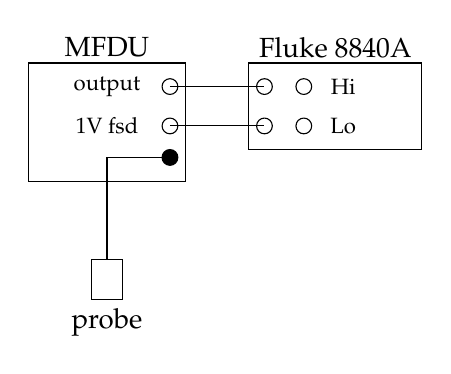
\begin{tikzpicture}
		\draw (0,0) rectangle (2,1.5);
		\draw (1.8, 1.2) circle (0.1);
		\draw (1.8, 0.7) circle (0.1);
		\draw[fill=black] (1.8, 0.3) circle (0.1);
		\draw (1.8, 0.3)--(1, 0.3);
		\draw (1,0.3)--(1,-1);
		\draw (0.8,-1)rectangle(1.2,-1.5);
		\draw node at (1, -1.8) {probe};
		\draw node at (1,1.2) {\footnotesize output};
		\draw node at (1,0.7) {\footnotesize 1V fsd};
		\draw node at (1, 1.7) {MFDU};
		\draw (1.8,1.2) -- (3, 1.2);
		\draw (1.8,0.7) -- (3, 0.7);
		\draw (2.8, 1.5) rectangle (5,0.4);
		\draw (3,0.7) circle (0.1);
		\draw (3,1.2) circle (0.1);
		\draw node at (3.9, 1.7) {Fluke 8840A};
		\draw (3.5,0.7) circle (0.1);
		\draw (3.5,1.2) circle (0.1);
		\draw node at (4, 1.2) {\footnotesize Hi};
		\draw node at (4, 0.7) {\footnotesize Lo};
	\end{tikzpicture}
	\caption{Oppsett for måling av magnetfeltstyrken. En probe er koblet inn i måleren for magnetisk flukstetthet (MFDU). For å lese av målingne bruker vi Fluke 8840A multimeter.}
	\label{fig:magnetfeltstyrke}
\end{figure}
Vi målte magnetfeltet inne i spolen mens den var tom. Vi målte også magnetfeltet med bare flaskebunnstativet på innsiden, før vi gjorde målinger med de forkjellige jernklumpene i spolen, konfigurert slik at de var rettet normalt på eller parallelt med magnetfeltet i spolen. Figur~\ref{fig:konfigurasjonerHall} viser de forskjellige konfigurasjonene i tillegg til de verdiene vi målte.

De forskjellige jernklumpene ble forsøkt plassert i sentrum av spolen, og måleproben ble plassert på toppen av jernklumpen.

Teoretisk (se appendiks~\ref{app:magspole}) forventer vi å ha

\begin{equation}
	B = \frac{\mu_0 I N}{L}=\frac{4\pi\cdot10^{-7}\cdot 5\cdot 244}{275\cdot 10^{-3}}\text{T}=5.57\text{mT}
	\label{eq:magfield}
\end{equation}
inne i spolen.

\subsubsection{Magnetisk fluks ved Faradays lov}
Faradays lov , ligning~\eqref{eq:max3}, kan brukes til å finne den magnetiske flukstettheten på en annen måte.

Vi benyttet følgende utstyr.
\begin{itemize}
	\item Strømgenerator
	\item Fluke 45, lokalnummer: 3193
	\item 2X PasPort Voltage-Current sensor
	\item datamaskin
	\item Primærspole, vindinger $N = 344$, lengde $L = 335$mm 
	\item Sekundærspole, vindinge r$n = 130$ , diameter $d = 6.5$mm 
	\item Spenningsintegrator
	%\item Linjal, Lyra 3112/50
\end{itemize}

Oppsettet med de forskjellige komponentene er vist i figur~\ref{fig:faradayEks}.
\begin{figure}[!ht]
	\centering
	\begin{circuitikz}
		%Strømgenerator
		\draw (0,0) rectangle (3,2);
		\draw (2.6, 0.4) circle (0.1);
		\draw (2.3, 0.4) circle (0.1);
		\draw (1.3, 0.4) circle (0.1);
		\draw (1.6, 0.4) circle (0.1);
		\draw node at (1.45, 0.8) {\centering skriv};
		\draw node at (2.45, 0.8) {\centering spole};
		\draw node at (1.5, 2.3) {\centering Strømgenerator};
		%Multimeter
		\draw (4,-1.2) rectangle (6,0);
		\draw (4.2, -0.8) circle (0.1);	
		\draw (4.5, -0.8) circle (0.1);	
		\draw (4.2, -0.5) circle (0.1);	
		\draw (4.5, -0.5) circle (0.1);	
		\draw node at (4.2, -1.4) {\centering com};
		\draw  (2.3,-0.8) to[L, l=\text{primær}] (4.2,-0.8);
		\draw (2.3, -0.8) -- (2.3, 0.4);
		\draw (2.6, 0.4) -- (4.5, 0.4);
		\draw (4.5, 0.4) -- (4.5, -0.5);
		\draw node at (5.5, 0.5) {\centering Fluke 45};
		%Integrator
		\draw (0.2, -4) rectangle (2, -2.5);
		\draw node at (1.1, -4.7) {\centering Integrator};
		\draw (0.5, -2) to[L, l=\text{sekundær}] (1.8, -2);
		\draw (0.4, -3.8) circle (0.1);
		\draw (0.7, -3.8) circle (0.1);
		\draw (1.8, -3.8) circle (0.1);
		\draw (1.5, -3.8) circle (0.1);
		\draw (1.8, -2) -- (1.8, -3.8);
		\draw (0.5, -2) -- (0.5, -3);
		\draw (0.5, -3) -- (1.5, -3);
		\draw (1.5, -3) -- (1.5, -3.8);
		%PasPort
		\draw (0.3, -1.0) rectangle (1.7, -0.5);
		\draw node at(1, -0.75) {\centering PasPort};
		\draw (1.6, 0.4) -- (1.6, -0.5);
		\draw (1.3, 0.4) -- (1.3, -0.5);
		\draw (0.4, -3.8) -- (0.4, -4.4);
		\draw (0.7, -3.8) -- (0.7, -4.2);
		\draw (0.7, -4.2) -- (3.5, -4.2);
		\draw (0.4, -4.4) -- (3.5, -4.4);
		\draw (1.7, -0.75) -- (1.9, -0.75);
		\draw (1.9, -0.75) -- (1.9, -1.2);
		\draw (1.9, -1.2) -- (3.5, -1.2);
		\draw (3.5, -1.2) -- (3.5, -2);
		\draw (3.5, -4.55) rectangle (4.9, -4.05); 
		\draw node at (4.2, -4.3) {\centering PasPort};
		\draw (4.2, -4.05) -- (4.2, -3);
		%Datamaskin
		\draw (3, -3) rectangle (6, -2);
		\draw node at (4.5, -2.5) {\centering Datamaskin};

	\end{circuitikz}
	\caption{Eksperimentelt oppsett for måling av magnetisk fluks ved Faradays lov. Sekundærspolen er kobbertråd surret rundt en jernstand. Denne legges inni primærspolen.}
	\label{fig:faradayEks}
\end{figure}
\subsection{Faradayeffekten}
\begin{figure}[!ht]
	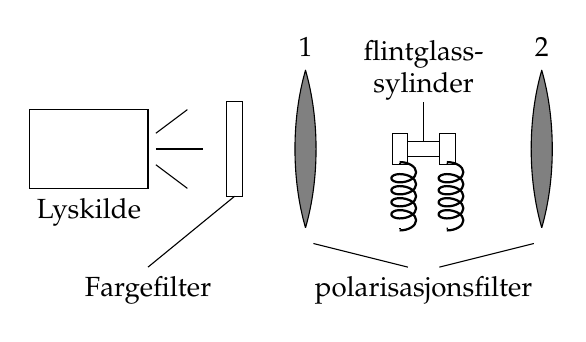
\begin{tikzpicture}
		\draw[line join=round,fill=black!50] (0.5,0) arc (-30:30:1 and 2) arc (150:210:1 and 2) ;
		\draw[line join=round,fill=black!50] (3.5,0) arc (-30:30:1 and 2) arc (150:210:1 and 2) ;
		\draw (-3, 0.5) rectangle (-1.5, 1.5);
		\draw (1.8,0.9) rectangle (2.2, 1.1);
		\draw (1.6, 0.8) rectangle (1.8, 1.2);
		\draw (2.2, 0.8) rectangle (2.4, 1.2);
		\draw (2.3, 0.8) to[L, l=](2.3, 0); 
		\draw (1.7, 0.8) to[L, l=](1.7, 0);
		\draw (-1.4, 1.2) -- (-1, 1.5);
		\draw (-1.4, 0.8) -- (-1, 0.5);
		\draw (-1.4, 1) -- (-0.8, 1);
		\draw node at (-2.25, 0.2) {\centering Lyskilde};
		\draw (-0.5, 0.4) rectangle (-0.3, 1.6);
		\draw (-0.4, 0.4) -- (-1.5, -0.5);
		\draw node at (-1.5, -0.8) {\centering Fargefilter};
		\draw (0.6, -0.2) -- (1.8, -0.5);
		\draw (3.4, -0.2) -- (2.2, -0.5);
		\draw node at (2, -0.8) {polarisasjonsfilter};
		\draw (2,1.1) -- (2, 1.6);
		\draw node at (2, 2.2) {flintglass-};
		\draw node at (2, 1.8) {sylinder};
		\draw node at (0.5, 2.3) {1};
		\draw node at (3.5, 2.3) {2};
	\end{tikzpicture}
	\caption{Oppsett for måling av Faradayeffekten. Spolenes plassering fører til at et magnetfelt som går langs sylinderens symmetriakse settes opp når det sendes strøm gjennom disse.}
	\label{fig:faradayoppsett}
\end{figure}
\section{Resultater}

\subsection{Diamagnetisme}
Tabell~\ref{tab:diameterVismut} viser målingene vi gjorde av diameteren til vismutstaven, gjennomsnittet og standardfeilen til disse målingene. Vi velger å bruke standardfeilen som usikkerheten i diameteren. Vi sitter da igjen med en diameter på $d = 10.2\pm0.1$mm.
\begin{table}[!ht]
	\centering
	\caption{Målinger og statistiske verdier for diameteren til vismutprøven.}
	\begin{tabular}{cc}
		\toprule
		\toprule
		& d[mm]\\
		\toprule
		&10.42\\ 
		&10.05\\
		&10.01\\
		&10.38\\
		&10.23\\
		\toprule
		{\textit mean()}& 10.22\\
		$\sigma_m$ & 0.08\\
		\toprule
	\end{tabular}
	\label{tab:diameterVismut}
\end{table}
%Usikkerheten i lengdenmålingen til vismutstangen estimerte vi til å være rundt \'en millimeter. Målingen vi gjorde gir oss da en lengde på $l = 10.1\pm0.1$cm.
\begin{table}
	\centering	
	\caption{Målinger av massen til vismut og legostangen, magnetfeltetet på toppen og bunnen av vismutstangen og strømmen påtrykt av strømforsyningen.}
	\begin{tabular}{cccc}
		\toprule
		\toprule
		$I$ [A] & vekt [g] & $B_2$[mT] & $B_1$[mT]\\
		\toprule
		0.0&	141.63&	1.4&	28 \\ 
		0.2&	141.63&	1.5&	119\\
		0.4&	141.63&	1.8&	204\\
		0.6&	141.59&	2.3&	286\\
		0.8&	141.57&	2.7&	362\\
		1.0&	141.53&	2.9&	433\\
		1.2&	141.48&	3.2&	498\\
		1.4&	141.43&	3.4&	555\\
		1.6&	141.38&	3.5&	608\\
		1.8&	141.35&	3.5&	653\\
		2.0&	141.32&	3.6&	690\\
		2.2&	141.29&	3.8&	722\\
		2.4&	141.26&	3.7&	748\\
		\toprule
	\end{tabular}
	\label{tab:measurements}
\end{table}
Vi målte magnetfeltet på toppen og bunnen av vismutstangen, og vekten til vismut- og legostangen, som funksjon av den påtrykte strømmen gjennom spolene. Resultatene er listet i tabell~\ref{tab:measurements}.

Et plot av kraften som virker på vismutstangen, grunnet det påtrykte magnetfeltet, som funksjon av kvadratet til magnetfeltet ved bunnen av stangen, finnes i figur~\ref{fig:lintilpass}. Denne figuren viser de eksperimentelle verdiene og en lineær tilpassing av disse. Utgangspunktet for kraften er målingene av massen til legostangen og vismutprøven. For å regne om til kraft satte vi tyngdens aksellerasjon til å være $g=9.82\text{m/s}^2$, og lot kraften være vekten trukket fra den maksimale vekten og multiplisert med tyngdens aksellerasjon.

\begin{figure}[!ht]
	\centering
	\includegraphics[width = 0.5\textwidth]{matlab/tilpasning.eps}
	\caption{Kraft som funksjon av kvadratet av magnetfeltets styrke. Eksperimentelle verdier markert med sirkler, og lineær tilpasning markert med stiplet linje.}
	\label{fig:lintilpass}
\end{figure}
Det interessante nå er ligningen for kraften. Denne har formen
\begin{equation}
	F_z = CB_1^2
	\label{eq:linear}
\end{equation}
hvor $C=-\chi\mathcal{A}/(2\mu_0)$ fra ligning~\eqref{eq:diaForenklet}.

Fra den lineære tilpassingen finner vi at $C = 0.0068\pm0.0002$N/T$^2$. Tverrsnittet av en sylinder er som kjent arealet av en sirkel, slik at
\begin{equation}
	\mathcal{A} = \frac{\pi d^2}{4}=\frac{\pi (10.2\cdot10^-3\text{m})^2}{4}=8.2\cdot10^{-5}\text{m}^2
	\label{eq:area}
\end{equation}

Vi har at $\mu_0=4\pi\cdot10^{-7}\text{N/A}^2$. Dette gir oss at 
\begin{equation}
	\chi = -\frac{2\mu_0 C}{\mathcal{A}}= -2.08\cdot 10^{-4}
	\label{eq:susecpt}
\end{equation}
Hvis vi ser bort fra usikkerheten i lineærtilpasningen og bruker at usikkerheten i målingen av magnetfeltet er omtrent $\Delta B = 5\%$, usikkerheten i massen er neglisjerbar og at usikkerheten i arealet $\Delta\mathcal{A}=\sigma_{m,d}/$\textit{mean(d)}$\approx1.6\%$ får vi susceptibiliteten til å være 
\begin{equation}
	\chi = -(2.08\pm0.21) \cdot 10^{-4}
	\label{eq:chiResult}
\end{equation}
Det er vanlig at andre kilder oppgir susceptibiliteten til vismut som $-1.66\cdot 10^{-4}$.
Hvis vi lineærtilpasser med resultatene for målingene uten å kvadrere magnetfeltet, får vi en relativ forskjell mellom målingene og tilpassingen som er større enn hvis vi kvadrerer. Den relative forskjellen mellom resultater og tilpassing er presentert i figur~\ref{fig:relativForskjell}. De tilhørende RMS-verdiene for avviket fra de målte til de tilpassede kreftene er $7.35\cdot 10^{-9}\text{N}^2$ og $1.30\cdot 10^{-7}\text{N}^2$, for henholdsvis magnetfelt kvadrert og ikke kvadrert.

\begin{figure}[!ht]
	\centering
	\includegraphics[width = 0.5\textwidth]{matlab/relativForskjell.eps}
	\caption{Relativ forskjell mellom de målte kreftene på vekten, og de vi finner ved å enten lineærtilpasse kraften til magnetfeltet eller til kvadratet av magnetfeltet.}
	\label{fig:relativForskjell}
\end{figure}
\subsection{Ferromagnetrisme}
Måleresultatene utført med Hall-sonden er presentert i figur~\ref{fig:konfigurasjonerHall}.
\begin{figure}[!ht]
	\centering
	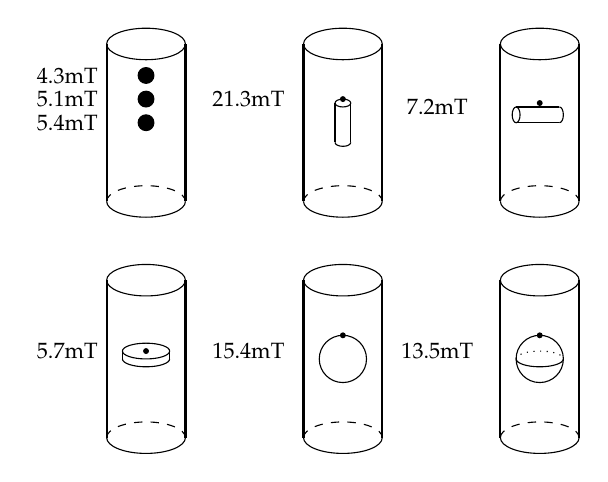
\begin{tikzpicture}
		\foreach \x in {1, 3.5, 6}{
			\foreach \y in {0, 3}{
				\draw (\x,\y+2) arc (180:360:0.5cm and -0.2cm);
				\draw (\x,\y+2) arc (180:360:0.5cm and 0.2cm);
				\draw (\x,\y) arc (180:360:0.5cm and 0.2cm);
				\draw [dashed] (\x,\y) arc (180:360:0.5cm and -0.2cm);
				\draw [thick,-] (\x,\y) -- (\x,\y+2);
				\draw [thick,-] (\x+1,\y) -- (\x+1,\y+2);
			}
		}			

		\draw [fill=black] (1.5, 4.0) circle (0.1);
		\draw [fill=black] (1.5, 4.3) circle (0.1);
		\draw [fill=black] (1.5, 4.6) circle (0.1);
		\draw node at (0.5,4.6) {\footnotesize 4.3mT};
		\draw node at (0.5,4.3) {\footnotesize 5.1mT};
		\draw node at (0.5,4.0) {\footnotesize5.4mT};

		%Jernstang vertikal
		\draw (3.9, 4.25) arc(180:360:0.1 and -0.05);
		\draw (3.9, 4.25) arc(180:360:0.1 and 0.05);
		\draw (3.9, 3.75) arc(180:360:0.1 and 0.05);
		\draw (3.9,3.75)--(3.9,4.25);
		\draw (4.1,3.75)--(4.1,4.25);
		\draw [fill=black] (4., 4.3) circle (0.03);
		\draw node at (2.8, 4.3) {\footnotesize 21.3mT};

		%Jernstang horisontal
		\draw (6.25, 4.1) arc(360:0:0.05 and -0.1);
		\draw (6.75, 4.2) arc (270:90:-0.05 and -0.1);
		\draw (6.2, 4.2) -- (6.75, 4.2);
		\draw (6.2, 4.0) -- (6.75, 4.0);
		\draw [fill=black] (6.5, 4.25) circle (0.03);
		\draw node at (5.2, 4.2) {\footnotesize 7.2mT};

		%Disk horisontal
		\draw (1.2,1.1) arc (180:360:0.3 and -0.1);
		\draw (1.2,1.1) arc (180:360:0.3 and 0.1);
		\draw (1.2,1.0) arc (180:360:0.3 and 0.1);
		\draw (1.2,1.0) -- (1.2, 1.1);
		\draw (1.8,1.0) -- (1.8,1.1);
		\draw [fill=black] (1.5, 1.1) circle (0.03);
		\draw node at (0.5, 1.1) {\footnotesize 5.7mT};

		%Disk vertikal
		\draw (4.0, 1) circle (0.3);
		\draw [fill=black] (4.0, 1.3) circle (0.03);
		\draw node at (2.8, 1.1) {\footnotesize 15.4mT};
		%Kule
		\draw (6.5, 1) circle (0.3);
		\draw (6.2, 1) arc (180:360:0.3 and 0.1);	
		\draw [dotted] (6.2, 1) arc (180:360:0.3 and -0.1);	
		\draw [fill=black] (6.5, 1.3) circle (0.03);
		\draw node at (5.2, 1.1) {\footnotesize 13.5mT};
	\end{tikzpicture}
	\caption{Resultater for målingene på innsiden av spolen med forskjellig formede objekter av ferromagnetisk materiale. Plasseingen av enden av proben for målingene er indikert med sorte prikker.}
	\label{fig:konfigurasjonerHall}
\end{figure}
Når vi målte magnetfeltet med flaskebunnstativet plassert inne i spolen målte vi en verdi på 5.3mT.

\subsection{Faraday-effekten}
\begin{table}
	\centering
	\caption{Tabell som viser dreiningsvinkelen for polarisasjonsfilter 2 i figur~\ref{fig:faradayoppsett}.}
	\begin{tabular}{cccc}
		\toprule
		\toprule
		& \multicolumn{3}{c}{$\theta$ for forskjellige $\lambda$ i $^\circ$} \\
		I[A] & $\theta_{440\text{nm}}$ & $\theta_{580\text{nm}}$ & $\theta_{595\text{nm}}$ \\
		\toprule
		-3.0 &	-4.2&	-4.6&	-4.0 \\
		-2.5&	-3.6&	-4.0&	-3.2 \\
		-2.0&	-3.2&	-3.0&	-2.2 \\
		-1.5&	-2.0&	-2.0&	-1.8 \\
		-1.0&	-0.8&	-1.2&	-1.0 \\
		0.0&	0.4&	0.4&	0.4 \\
		1.0&	1.8&	2.2&	1.8 \\
		1.5&	2.6&	3.0&	2.8 \\
		2.0&	3.8&	3.8&	3.4 \\
		2.5&	4.2&	5.0&	4.4 \\
		3.0&	5.2&	5.6&	4.8 \\
		\toprule
	\end{tabular}
	\label{tab:<+label+>}
\end{table}<++>
\section{Diskusjon}

\printbibliography
\clearpage
\onecolumn
\appendix

%\section{Vedlegg}

\section{Magnetfelt gjennom spole}
\label{app:magspole}
Betrakter vi ligning~\eqref{eq:max4} og antar at det elektriske feltet ikke endrer seg med tid, så sitter vi igjen med 
\begin{equation}
	\nabla\times\mathbf{B} = \mu_0\mathbf{J}
	\label{eq:independentOfTime}
\end{equation}
Vi kan nå benytte Stokes teorem til å gjøre om integralet slik at
\begin{align}
	\int_\Omega (\nabla\times\mathbf{B})\cdot d\mathbf{a} = \oint_\mathcal{C}\mathbf{B}\cdot d\mathbf{r}=\mu_0\int_\Omega \mathbf{J} \cdot d\mathbf{a} 
	\label{}
\end{align}
der $d\mathbf{r}$ er den infenitesimale tangentvektoren til kurven $\mathcal{C}$. 

Benytter vi ligning~\eqref{eq:currentDensity} så sitter vi igjen med 

\begin{align}
	\oint_\mathcal{C}\mathbf{B}\cdot d\mathbf{r}=\mu_0 I_\text{omfavnet}
	\label{eq:etterStokes}
\end{align}
der $I_\text{omfavnet}$ er den totalle strømmen som går gjennom flaten omsluttet av den lukkede kurven $\mathcal{C}$.

Vi ser nå på en spole, et tilfelle som er skissert i figur~\ref{fig:spole}. Det magnetiske feltet er tilnærmet null utenfor spolen, og strømmen som går gjennom flaten omsluttet av den lukkede kurven er antall vindinger, $N$, multiplisert med strømmen vi har gjennom spolen.

Siden vi bare har bidrag til det magnetiske feltet langs symmetriaksen til spolen, så reduseres integralet til enkel multiplikasjon. Vi sitter igjen med
\begin{equation}
	BL = \mu_0IN \implies B = \frac{\mu_0 I N}{L}
	\label{eq:magSpole}
\end{equation}

\begin{figure}[!ht]
	\centering
	\begin{tikzpicture}
    % Define a formula for the coil.
    % This is what the numbers mean:
    % 0.3 ... how far the rings are apart
    % 0.4 ... how much from the side the rings are seen (try 0 and the same as the radius)
    % 1.5 ... radius of the rings
		\def\coil#1{
			{0.3 * (2*#1 + \t) + 0.4*sin(\t * pi r))},
			{1.5 * cos(\t * pi r)}
		}

    % Draw the part of the coil behind the rectangle
		\foreach \n in {0,1,...,10} {
			\draw[domain={0:1},smooth,variable=\t,samples=15]
			plot (\coil{\n}); 
		}

    % Draw the rectangle
		\draw[-<-=0.80, dashed](-0.5,-2) rectangle (7,0);
		\node (curve) at (3.5, -2.5) {$\mathcal{C}$};

    % Draw the part of the coil in front of the rectangle
		\draw[->-=0.3, domain={1:2},smooth,variable=\t,samples=15,
			preaction={draw,white,line width=3pt}     % remove if undesired
		] node at (-0.3, -0.5)  {$I$}
		plot (\coil{0});
		\foreach \n in {1,2,...,10} {
			\draw[domain={1:2},smooth,variable=\t,samples=15,
				preaction={draw,white,line width=3pt}     % remove if undesired
			]
			plot (\coil{\n});
		}
		\draw[very thick, ->] (2.5,0) -- (4.5,0);
		\node (field) at (3.9, 0.3) {$\mathbf{B}$};
		\node (surface) at (6, -1.7) {$\Omega$};
	\end{tikzpicture}

	\caption{Figur som viser spole og valgt integrasjonskurve for ligning~\ref{eq:etterStokes}. Integrasjonskurven ligger langs symmetriaksen til spolen.} 
	\label{fig:spole}
\end{figure}

\end{document}




